\chapter{Along Came Clojure}
\label{chap:along-came-clojure}
	In this chapter we further discuss our implementation.  In \cref{sec:basic-principles-fp} we discuss the basic tenets of functional programming with an emphasis on how Clojure implements these tenets.  Further attention is paid to how Clojure uses these tenets to implement its concurrency model.
	
	In \cref{sec:search-with-clojure} we illustrate how Clojure's \gls{jvm} interoperability is used to interface with Lucene and \gls{jdbc} drivers in order to perform indexing and search on data.  This section also covers keyword as well as graph search in document space.
	
	\section{Basic Principles of Functional Programming}
	The functional programming paradigm follows a handful of basic tenets; values are immutable, and functions must be free of side-effects \cite{fp-89}.
	
	The first tenet, that values are immutable, refers to the fact that once a value is bound, this value may not change.  In procedural programming there is the concept of assignment, whereas in functional programming, a value is bound.  Assignment allows a value to change, binding does not.
	
	Immutable values are advantageous as they remove a common source of bugs; state must explicitly be changed.  This removes the ability for different areas of a program to modify the state (i.e.~global variables).
	
	Unfortunately immutable values can also lead to inefficiency.  For example, in order to add a key-value pair to a map, an entirely new map must be created with the existing key-value pairs copied to it.  In practice this is avoided through the use of persistent data structures with multi-versioning.
	
	The second tenet, that functions must be free of side-effects, means that the output of a function must be predictable for any given input.  This purity reduces a large source of bugs, and allows out-of-order execution. \cite{fp-89}.

	\subsection{Features of Clojure}
	\label{sec:features-of-clojure}
		The creator of Clojure, Rich Hickey, describes his language as follows:
		
		\begin{displayquote}[\cite{clj-home}]
			Clojure is a dialect of Lisp, and shares with Lisp the code-as-data philosophy and a powerful macro system.  Clojure is predominantly a functional programming language, and features a rich set of immutable, persistent data structures.  When mutable state is needed, Clojure offers a software transactional memory system and reactive Agent system that ensure clean, correct, multithreaded designs.
		\end{displayquote}
		
		As the above quote describes, Clojure follows the basic tenets of functional programming.
		
		\subsubsection{Immutable, Persistent Data Structures}
			Clojure supports a rich set of data structures.  These are immutable, satisfying the first tenet, as well as persistent, in order to overcome the inefficiency described previously.
			
			The provided data structures range from scalars (numbers, strings, characters, keywords, symbols), to collections (lists, vectors, maps, array maps, sets) \cite{clj-data-structures}.  These data structures are sufficient enough to allow us to use the universal design pattern \cite{udp-08}.
			
			Clojure also has the concept of persistent data structures.  These are used in order to avoid the inefficiency of creating a new data structure and copying over the contents of the old data structure simply to make a change.  Clojure creates a skeleton of the existing data structure, inserts the value into the data structure, then retains a pointer to the old data structure.  If an old property is accessed on the new data structure, Clojure follows the pointers until the property is found on a previous data structure.
			
			\begin{figure}
				\centering
				
				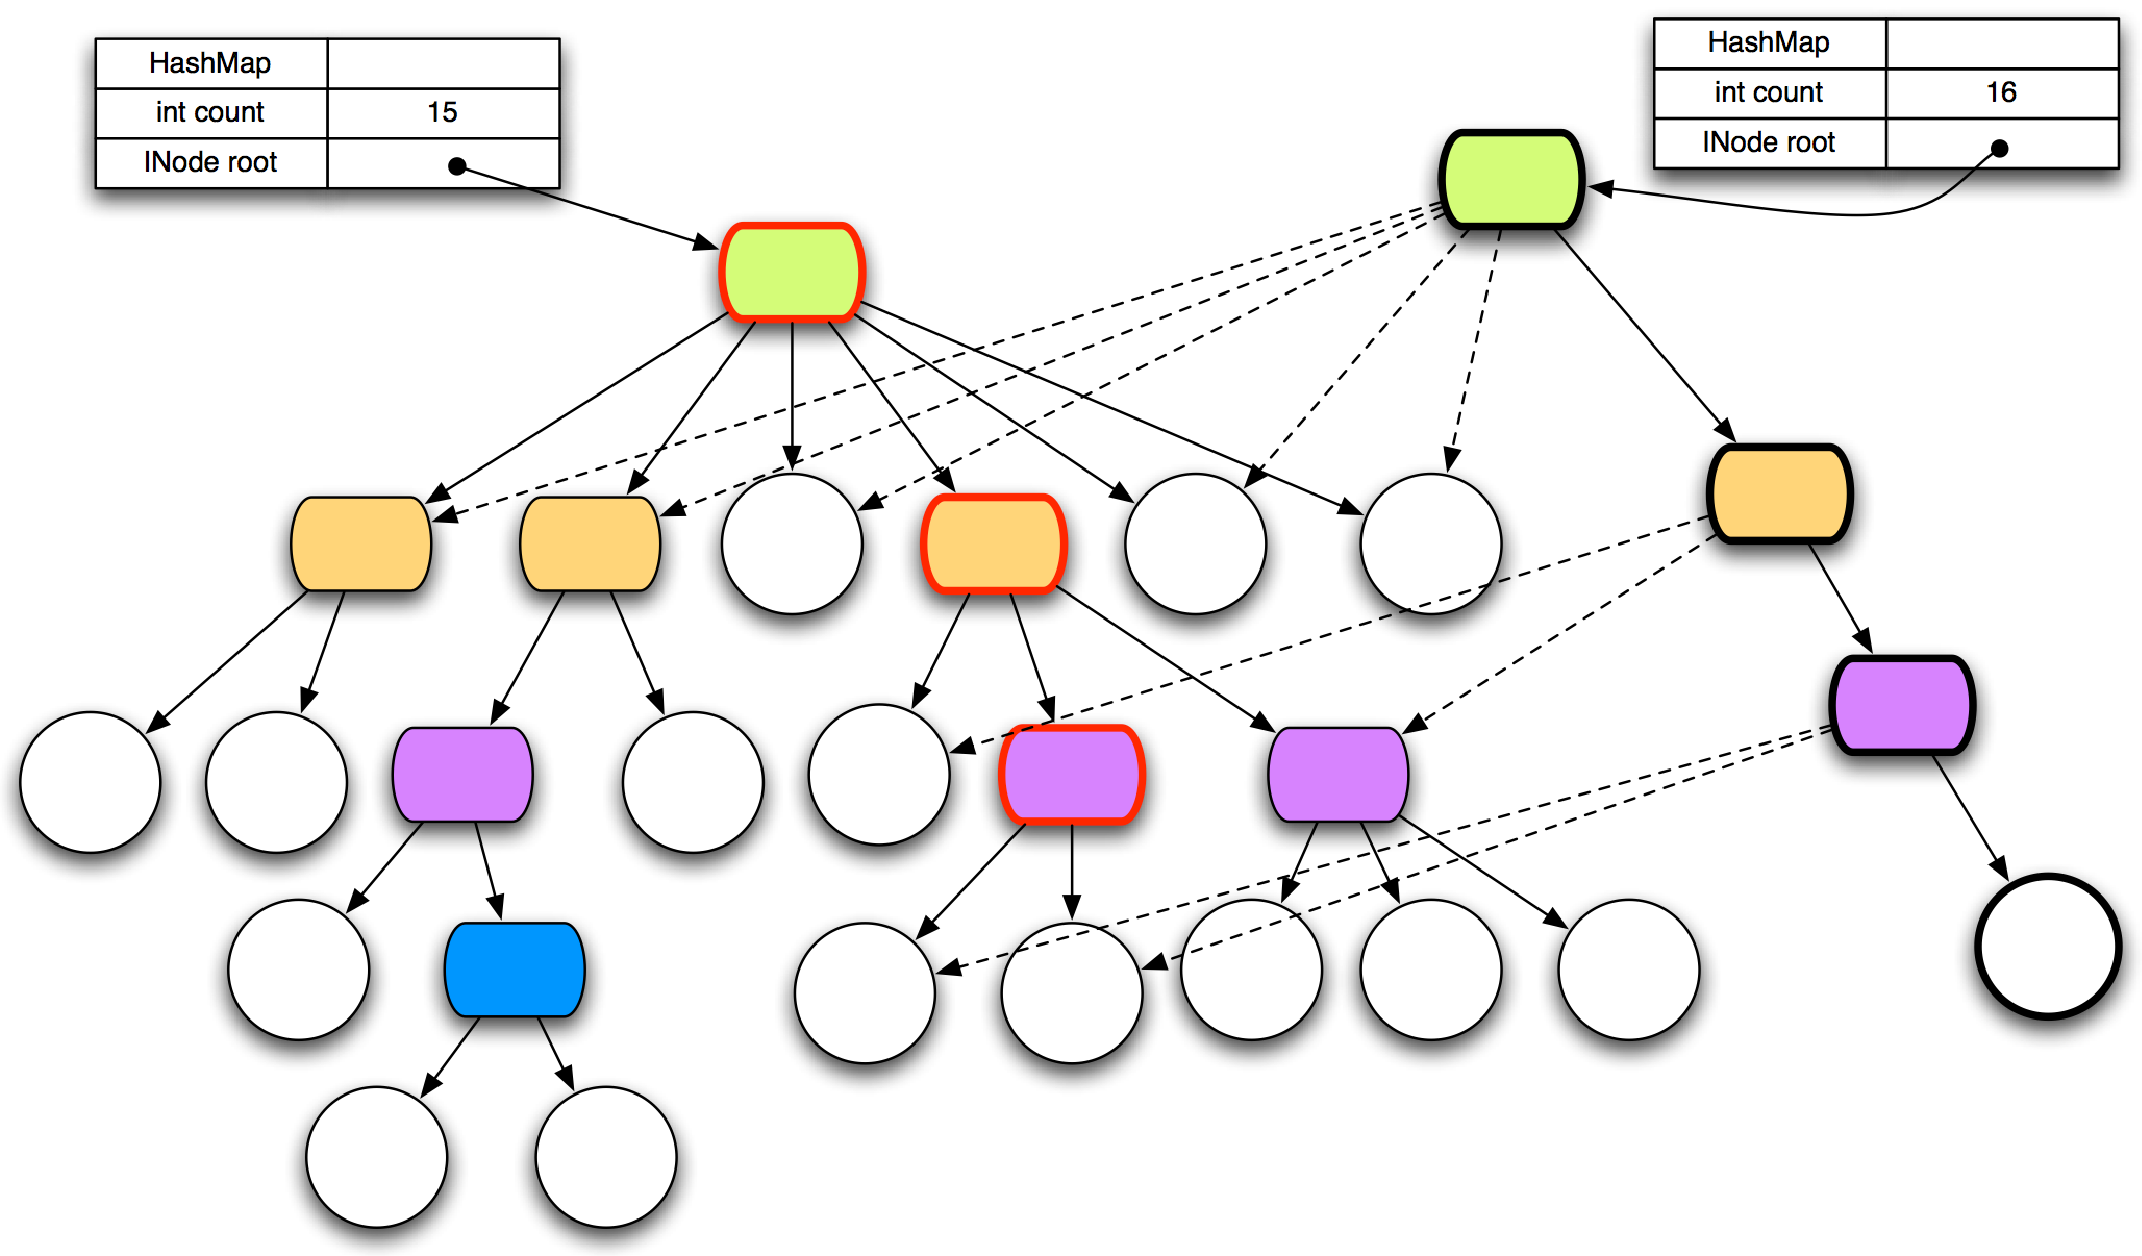
\includegraphics[scale=0.42]{figures/diagrams/persistent-data-structure}
				
				\caption{Representation of how data structures are ``changed'' in Clojure (Source:  \cite{clj-persistent})}
				\label{fig:persistent-data-structure}
			\end{figure}
			
			In \vref{fig:persistent-data-structure}, we see what happens when a persistent data structure is ``changed'' in Clojure.  The root of the left tree is the data structure before, and the root of the right tree is the data structure after.  Note how the changed map retains pointers to all but the updated value; the newly created value is pointed to instead of the previous one.
		
		\subsubsection{Concurrency}
			Clojure supports four systems for concurrency:  \gls{stm}, agents, atoms, and dynamic vars.  The differences between these systems are summarized in \vref{tbl:concurrency-system-comparison}.
			
			\begin{table}
				\centering
				
				\begin{tabular}{llll}
					\toprule
					System Name & Synchronous & Coordinated & Scope \\
					\midrule
					\gls{stm} & Yes & Yes & Application \\
					Agents & No & No & Application \\
					Atoms & Yes & No & Application \\
					Dynamic Vars & Not Applicable & Not Applicable & Thread \\
					\bottomrule
				\end{tabular}
				
				\caption{Comparison between Clojure's four systems for concurrency}
				\label{tbl:concurrency-system-comparison}
			\end{table}
			
			\todo{More concurrency}
			
		\subsubsection{Interoperability With the \gls{jvm}}
			\todo{Compare to other functional languages with decent library support}
			Traditionally, functional programming languages have been undesirable for numerous reasons:  compatibility, libraries, portability, availability, packagability, and tools \cite{no-fp-98}.  Clojure attempts to avoid many of these reasons by running on the \gls{jvm}.  The \gls{jvm} allows Clojure to both call and be called by Java and other languages.  It includes syntactic sugar -- features of a language added in order to simplify the language from a human perspective -- to transparently call Java code, as well as make itself available to Java.  This avoids the above issues.
			
			The syntactic sugar provided by Clojure allows for the accessing of object members, the creation of objects, the calling of methods on an instance or class, etc.  Clojure also includes shortcuts to perform multiple operations on the same object.  The syntax is given in \vref{tbl:jvm-interop-syntax}.
			
			\begin{table}
				\centering
				
				\begin{tabular}{lll}
					\toprule
					Operation & Form & Example \\
					\midrule
					Member Access & \texttt{(.<member> <obj> [args])} & \texttt{(.toString 5)} \\
					 & \texttt{(. <obj> <member> [args])} & \texttt{(. 5 toString)} \\
					 & \texttt{(<class>/<member> [args])} & \texttt{(Integer/parseInt ``5'')} \\
					Object Instantiation & \texttt{(<class>. [args])} & \texttt{(Integer. 5)} \\
					 & \texttt{(new <class> [args])} & \texttt{(new Integer 5)} \\
					Multiple Operations & \texttt{(doto <obj> [forms])} & \texttt{(doto (Vector.) (.add 1))} \\
					\bottomrule
				\end{tabular}
				
				\caption{Syntactic sugar for \gls{jvm} interoperability}
				\label{tbl:jvm-interop-syntax}
			\end{table}
			
			We utilize Clojure's \gls{jvm} interoperability to make use of Apache Lucene and \gls{jdbc}.
			
			\begin{figure}
				\begin{singlespaced}
					\begin{pygments}{clj}
(defn ^Directory idx-path
  [path]
  (-> path File. SimpleFSDirectory.))
					\end{pygments}
				\end{singlespaced}
				
				\caption{Clojure code that, given a path, returns a \texttt{Directory} object}
			\end{figure}
	\section{Search With Clojure}
\label{sec:search-with-clojure}
	Clojure's excellent \gls{jvm} interoperability permits the use of countless third-party libraries.  The most extensively used was Lucene.
	
	\subsection{Full-Text Search Using Lucene}
		\textcquote{luc-home}{Apache Lucene\texttrademark\ is a high-performance, full-featured text search engine library written entirely in Java.}  Lucene implements the Document Model (\cref{sec:document-model}), providing a simple yet powerful \gls{api} to perform full-text search.  Among these features is the ability to vectorize documents according to the Vector Space Model (\cref{sec:vectorization-of-documents}), utilize the extended document model to provide semi-structured documents (\cref{sec:extending-the-document-model}), and issue search queries against the index (\cref{def:search-query}).
	
	\subsection{Indexing Relational Database}
		The indexing of relational objects is a complicated process.  The objects must be retrieved from the relational database, transformed from named tuples into documents, then placed in the index.  Additionally, all foreign keys (\cref{def:foreign-keys}) must be encoded as documents (\cref{sec:encoding-entity-group-as-document-group}) in order to satisfy \cref{sec:mapping-entity-groups-to-documents}.
		
		The schema graph (\cref{def:schema-graph}) must be defined before the relational database may be crawled.
		
		\subsubsection{Schema Graph Definition}
		\label{sec:entity-schema}
			The schema graph is defined using Korma, which \textcquote{clj-korma}{is a \gls{dsl} for Clojure}.  Each schema component, whether an entity or entity group, is defined by \texttt{EntitySchema} records.  Each record accepts a map which specifies how each class of document should be indexed and identified.  The keys of this map are given in \vref{tbl:entity-schema-keys}.
			
			\begin{table}
				\centering
				
				\begin{tabular}{lp{9cm}l}
					\toprule
					Key & Description & Type(s) \\
					\midrule
					\texttt{:T} & Entity (\texttt{:entity}) or entity group (\texttt{:entity}) & Symbol \\
					\texttt{:C} & Table name for entities, brief description for entity groups & Symbol or String \\
					\texttt{:sql} & \Gls{sql} query used to construct the entity or entity schema & Expression \\
					\texttt{:ID} & Attribute or attributes that comprise the key (\vref{def:keys}) & Symbol or list of symbols \\
					\texttt{:attrs} & List of attributes to analyze to fields & List of symbols \\
					\texttt{:values} & List of attributes to index as values, must be subset of \texttt{:attrs} & List of symbols \\
					\bottomrule
				\end{tabular}
				
				\caption{Keys expected by \texttt{EntitySchema} records}
				\label{tbl:entity-schema-keys}
			\end{table}
		
		\subsubsection{Crawling the Relational Database}
			With the schema graph defined, the system is able to crawl the relational database, yielding a sequence of named tuples.  It iterates through every \texttt{EntitySchema} record, instructing every record to crawl itself given a database connection and index writer (\vref{clj:building-the-index}).
			
			\begin{figure}
				\begin{singlespaced}
					\begin{pygments}{clj}
(doseq [ent-def schemas]
  (crawl ent-def db-conn idx-w))
					\end{pygments}
				\end{singlespaced}
				
				\caption{Building the index}
				\label{clj:building-the-index}
			\end{figure}
			
			The \texttt{Database} protocol provides an \texttt{execute-query} method that permits access to the database.  In the current implementation, the \texttt{Sqlite3} record implements the \texttt{Database} protocol.  This record issues the query as-is, applying a given function to every result.
			
			Each record issues a \gls{sql} query against the database that retrieves all named tuples that it represents.  This query is given by the \texttt{:sql} key of the record.  For every symbol defined by the \texttt{:values} key, an additional query is issued.  These queries retrieve all distinct (within the context of that relation and attribute) values.
		
		\subsubsection{Transformation}
			For every named tuple, a document is constructed (see \cref{sec:named-tuples-documents}).  In addition to the attributes, several other fields may be added to the document.  These special fields contain additional meta information about the document.  For example, the class, type, and unique identifier are added to an entity, while an entity group has a space-delimited list of unique identifiers that comprise the group.
			
			Before becoming a document, named tuples are transformed into an internal representation.  The internal representation adds flexibility to the system; so long as functions exist to convert between the internal representation and other forms, the system does not care about the source.
			
			Clojure permits the annotation of data with metadata.  Named tuples are returned as maps, with key-value pairs representing attributes and values for each tuple.  Metadata may be associated with a named tuple that does not affect its key-value pairs.
			
			The map of attributes and values of a named tuple is annotated with the function \texttt{(with-meta obj map)}.  The \texttt{obj} parameter is the named tuple, while \texttt{map} is a map of metadata as defined by the system.  The keys of \texttt{map} for each type (value, entity, or entity group) are defined in \vref{tbl:type-metadata}.
			
			\begin{table}
				\begin{subtable}[b]{0.33\linewidth}
					\centering
					
					\begin{tabular}{ll}
						\toprule
						Key & Value \\
						\midrule
						:type & :value \\
						:class & <rel>|<attr> \\
						\bottomrule
					\end{tabular}
					
					\caption{Value}
				\end{subtable}
				\begin{subtable}[b]{0.33\linewidth}
					\centering
					
					\begin{tabular}{ll}
						\toprule
						Key & Value \\
						\midrule
						:type & :entity \\
						:class & <rel> \\
						:ID & <rel>|<pk> \\
						\bottomrule
					\end{tabular}
					
					\caption{Entity}
				\end{subtable}
				\begin{subtable}[b]{0.33\linewidth}
					\centering
					
					\begin{tabular}{ll}
						\toprule
						Key & Value \\
						\midrule
						:type & :group \\
						:entities & <rel>|<pk> \\
						 & [<rel>|<pk> \ldots] \\
						\bottomrule
					\end{tabular}
					
					\caption{Entity Group}
				\end{subtable}
				
				\caption{Metadata associated with each type}
				\label{tbl:type-metadata}
			\end{table}
			
			The internal representation of the named tuple given in \vref{tbl:hmr-properties} is given in \vref{clj:with-meta-internal-rep}.
			
			\begin{figure}
				\begin{singlespaced}
					\begin{pygments}{clj}
(with-meta
  {:code    "CDPS 101"
   :title   "Human-Mutant Relations"
   :subject "CDPS"}
  {:type  :entity
   :class :course
   :id    "course|cdps_101"})
					\end{pygments}
				\end{singlespaced}
				
				\caption{Internal representation of named tuple from \vref{tbl:hmr-properties}}
				\label{clj:with-meta-internal-rep}
			\end{figure}
			
			Once the internal representation is constructed, it may be transformed into a document.  The mapping of a map to document is trivial; a field is created for every key in the map and the value corresponding to the key is the value of the field.  Unfortunately Lucene does not facilitate the storage of metadata.  Therefore the system must deal with metadata in a different way.
			
			The system modifies each key of the metadata; two underscores are prepended and appended to the key name.  This allows the system to differentiate between metadata and attributes.  The transformation from internal representation to document is given in \vref{tbl:internal-rep-to-document}.
			
			\begin{table}
				\centering
				
				\begin{tabular}{ll}
					\toprule
					Field & Value \\
					\midrule
					code & cdps 101 \\
					title & human mutant relations \\
					subject & cdps \\
					\_\_type\_\_ & entity \\
					\_\_class\_\_ & course \\
					\_\_id\_\_ & course|cdps\_101 \\
					\bottomrule
				\end{tabular}
				
				\caption{Document of internal representation from \vref{clj:with-meta-internal-rep}}
				\label{tbl:internal-rep-to-document}
			\end{table}
		
		\subsubsection{Indexing}
			With the named tuples transformed into documents, the index may be constructed.  The first step is to open the index for writing.  In Lucene, this is accomplished by creating an \texttt{IndexWriter} object on a \texttt{Directory} object that points to the index location.  The \texttt{IndexWriter} object also expects an analyzer to be used by default on documents it indexes.  The system uses a \texttt{WhitespaceAnalyzer} by default.
			
			For every named tuple, the transformed document is written to the index by the index writer object.  In addition, the indexing document (\cref{sec:encoding-entity-group-as-document-group}) of every entity group is added.
		
	\subsection{Keyword Search in Document Space}
	\label{sec:keyword-search-document-space}
		With the entity graph encoded into the document model, users may begin issuing search queries.  Every query follows the following pattern:  users look up values (optionally using fuzzy search), these values are used to locate entities, and once two entities are selected, the system attempts to locate connections between the two.
		
		\subsubsection{Fuzzy Value Search}
			Recall that entity values are stored as their \(n\)-gram (\cref{sec:n-gram}).  This allows users to make character substitutions, deletions, or additions, and still return values they may have intended on finding.  Without the use of \(n\)-grams, a misspelling on the user's part would result in either no or irrelevant values being returned.  Values that are approximately matched would be assigned a lower score than those which are fully matched, but they would at least appear in the results.
			
			Rather than guessing the user's intention, the system presents the user with a list of values in order to give them the option of substituting their entry for an approximate match.  This autosuggest feature is intended to improve the user experience by eliminating a source of frustration -- irrelevant results as a result of a simple spelling error.
		
		\subsubsection{Flexible Keyword Search \gls{api}}
			The system provides a simple -- yet flexible -- keyword search \gls{api}.  Recall the extended query (\cref{ex:extended-query}) is in the form
			\[
				\query(\field, \w)
			\]
			
			The search \gls{api} provides a function that accepts a symbol defining the field to search in, as well one or more words to search for.  A phrase query comprised of every word is constructed.
			\[
				\query(\field, \w_1, \w_2, \dotsc, \w_n) = \bigcap_{\w \in \{\w_1, \w_2, \dotsc, \w_n\}} \query(\field, \w)
			\]
			
			Another function, \texttt{boolean-query}, accepts one or more \(\query\) functions as well as a boolean operator for each and returns the result.  The symbols \texttt{:and}, \texttt{:or}, and \texttt{:not} provide \(\cap\), \(\cup\), and \(\neg\), respectively.
			
			\begin{ex}[\texttt{boolean-query}]
				For example, the query in \cref{ex:extended-query} is given in \vref{clj:boolean-query}.
				
				\begin{figure}
					\begin{singlespaced}
						\begin{pygments}{clj}
(boolean-query
 [[:and (query :subject ``MATH'')]
  [:and (query :text ``class'')]])
						\end{pygments}
					\end{singlespaced}
					
					\caption{Boolean query in Clojure}
					\label{clj:boolean-query}
				\end{figure}
			\end{ex}
		
		\subsubsection{Translation of Search Results to Relational Space}

	\subsection{Graph Search in Document Space}
		With the ability for users to find relevant entities using fuzzy value search and the flexible keyword search \gls{api} (\cref{sec:keyword-search-document-space}), they must be able to find connections between two entities.  As stated previously (\cref{clm:lossless}), the document encoding of relational data is a graph.  This allows the system to search for links between entities by utilizing one or more graph search algorithms, such as \gls{bfs}.
		
		\begin{figure}
			\centering
			
			\begin{dot2tex}[dot]
digraph G {
node [shape=plaintext]; "Human-Mutant Relations"; "Community Development & Policy Studies";

"Human-Mutant Relations" -> "Community Development & Policy Studies";
}
			\end{dot2tex}
			
			\caption{Human-Mutant Relations entity group}
			\label{fig:hmr-entity-group}
		\end{figure}
		
		\subsubsection{Why We Need Graph Search}
			Tuples are fragments, or facts, of larger pieces of knowledge.  By utilizing graph search, we amalgamate these facts to provide a user with a broader view.
			
			\begin{ex}
				By utilizing graph search, we can take the facts in \cref{tbl:facts} and compose new facts.  For example, we could learn who teaches Complex Analysis.  It also allows us to ask questions, such as ``who taught Complex Analysis with Instructor X?''
				
				\begin{table}
					\begin{subtable}[b]{0.5\linewidth}
						\centering
						
						\begin{tabular}{ll}
							\toprule
							Field & Terms \\
							\midrule
							code & \(\{\text{math}, \text{360}\}\) \\
							title & \(\{\text{complex}, \text{analysis}\}\) \\
							subject & \(\{\text{math}\}\) \\
							\bottomrule
						\end{tabular}
						
						\caption{Fact representing a Course}
						\label{subtbl:fact-course}
					\end{subtable}
					\begin{subtable}[b]{0.5\linewidth}
						\centering
						
						\begin{tabular}{ll}
							\toprule
							Field & Terms \\
							\midrule
							id & \(\{\text{math}\}\) \\
							name & \(\{\text{mathematics}\}\) \\
							\bottomrule
						\end{tabular}
						
						\caption{Fact representing a Subject}
						\label{subtbl:fact-subject}
					\end{subtable}
					
					\caption{Fragments, or facts, of information in a dataset}
					\label{tbl:facts}
				\end{table}
			\end{ex}
			
			This automated discovery of relations between facts is why graph search is important.
		
		\subsubsection{Graph Search Algorithms}
			Recall we defined a graph as \(G = (V, E)\), where \(V\) is the set of all facts in the database, and \(E\) is the set of relations between facts.
		
		\subsubsection{Graph Search in Document Space}
			
		
		Graph search algorithms
		=======================
		
		%# Definition of the graph
		
		G = (V, E)
		
		V = all entity-groups in DB
		Let $Ent(v)$ be the set of entities in entity group $v$.
		We say that two vertices in $G$ are connected if and only if:
		
		$Ent(v)\cap Ent(v')\not=\emptyset$.
		
		%# Definition of graph search
		
		Given a keyword query q, find a subgraph, $H$, of G to:
		- minimize the vertices in H
		- maximize the satisfaction of keywords in $q$ by vertices in $H$.
		
		Example (based on UOIT or superhero) should be given here.
		- just use the canonical example for benchmark testing.
		
		%# Logical specification of the graph search algorithm:
		
		- find all vertices by entity group search, and call this C.
		- use any graph search algorithm to minimally connect the vertices in C
		as follows. 
		let s\in C be a source.
		for each t\in C-{s}:
		find path connecting s->t such that len(path) <= user-defined-bound.
		
		%# Why use document space for graph search (THESIS OF YOUR THESIS)
		
		- finding the relevant "seed" vertices is really fast.  This is done by
		using full text search on the documents of an entity graph.  Therefore, it
		allows fuzzy search for the seeds.
		- finding connected entity groups is really fast - this is done by using the
		indexing document.  Using a single keyword query, we can find all relevant
		entity groups in the database.
		
		Example: spell this out:
		
		index-doc(v0) = student:ABC, course:XYZ
		query: (:or (:and (id:ABC) (C:student)) 
		(:and (id:XYZ) (C:course)))
		
		%# Breadth-first search
		
		Description: copy this from CLRS
		<Richard>
		
		Functional description of BFS
		
		Distributed functional description of BFS
		
		Implementation details:
		- Ref
		- Atoms
		- Agent
		
		\begin{itemize}
			\item Why we need graph search
			\item Search in document graph using graph search algorithms with functional implementations: (Ford Fulkerson, BFS)
			\item Speed up using concurrency
			\item Clojure specific optimization: ref + atom
		\end{itemize}
	
	\section{Web Interface}
	\label{sec:web-interface}
		In order to make the system more accessible to novice users, a web-based interface was created.
		
		The first step involves searching for entities by a value.  We use approximate (\(n\)-gram) string matching to find relevant values despite potential character substitutions, deletions, or additions.
		
		\begin{figure}[H]
			\centering
			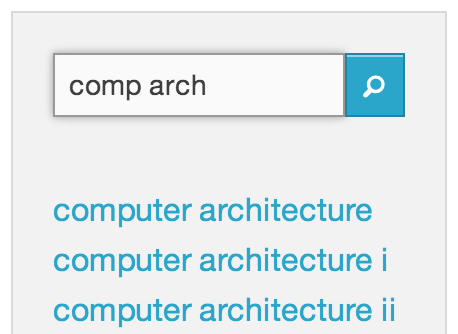
\includegraphics[scale=0.5]{figures/images/step-1}
			
			\caption{Approximate string matching of values}
			\label{fig:webui-step-1}
		\end{figure}
		
		Entities that match the desired values are displayed to the user.  They have the option of specifying the entity as either the source, or the target.
		
		\begin{figure}[H]
			\centering
			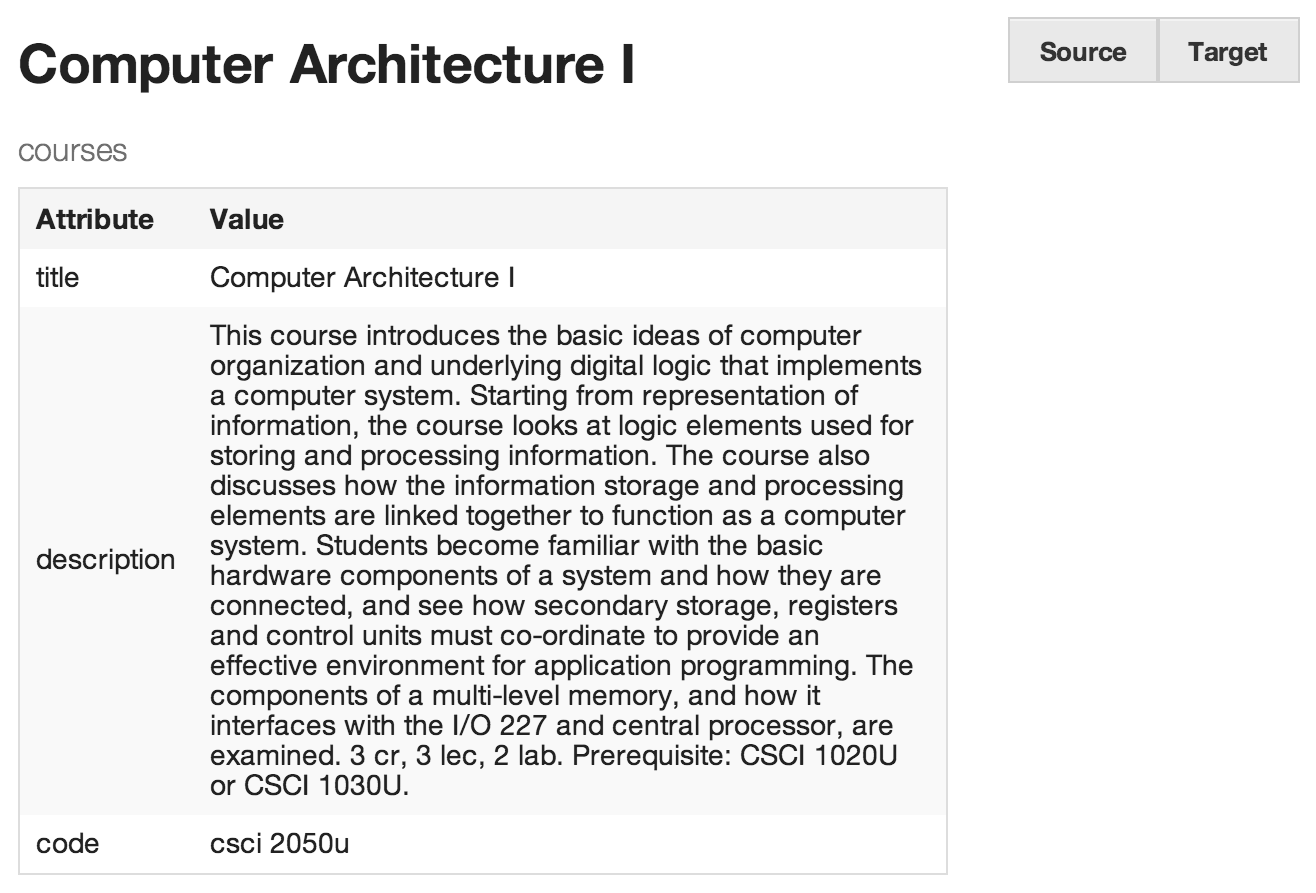
\includegraphics[scale=0.5]{figures/images/step-2}
			
			\caption{Tabular display of entities}
			\label{fig:webui-step-2}
		\end{figure}
		
		When an entity is chosen, the navigation bar at the top of the page is updated to reflect the new selection.  This allows the user to hover their cursor over the respective element in order to remind themselves of their selection.
		
		\begin{figure}[H]
			\centering
			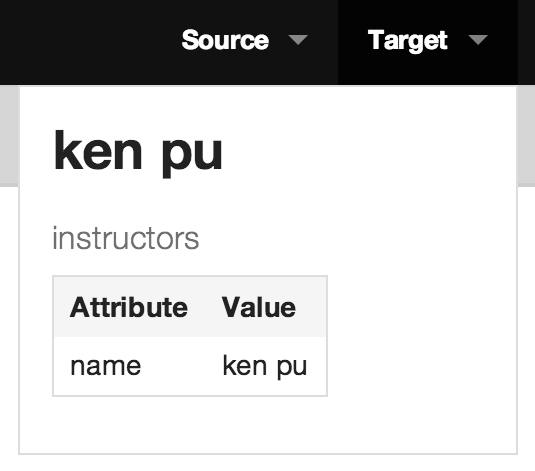
\includegraphics[scale=0.5]{figures/images/step-3}
			
			\caption{Chosen entities are displayed at the top}
			\label{fig:webui-step-3}
		\end{figure}
		
		When both a source and target entity are selected, the user is able to search for the shortest path between them.  They are given the option of which graph search algorithm implementation to use.
		
		\begin{figure}[H]
			\centering
			
\includegraphics[scale=0.5]{figures/images/step-4}
			
			\caption{The algorithm implementation may be selected}
			\label{fig:webui-step-4}
		\end{figure}
		
		A short message displaying the search duration as well as memory consumption is followed by a series of tables representing the intermediate entities between the source and target entities.
		
		\begin{figure}[H]
			\centering
			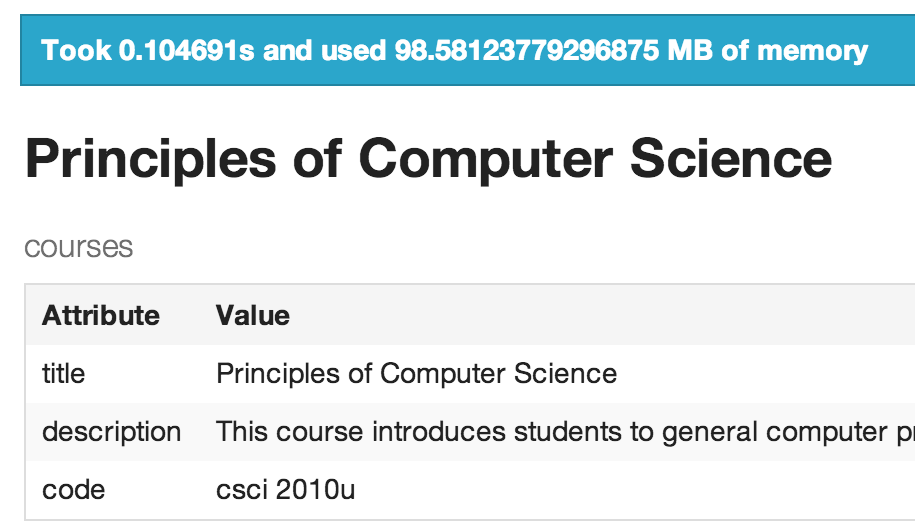
\includegraphics[scale=0.5]{figures/images/step-5}
			
			\caption{Result of a search between entities}
			\label{fig:webui-step-5}
		\end{figure}
		
		This interface allows users to query the database for information in a familiar manner.